Nathan é um menino apaixonado por triângulos, por conta disso em sua casa só tem vasilhas triangulares. Contudo, sua mãe Ana sempre faz panquecas circulares para o seu filho levar para escola. Como Nathan é ruim em matemática ele nunca sabe qual o melhor recipiente para levar. Por sorte no seu material escolar há uma régua, conseguindo dessa forma medir os lados de todas as vasilhas da casa. Sendo assim, o seu trabalho 
será criar um programa que lê as medidas de Nathan e mostrá-lo quais são os raios limites que a panqueca pode ter para cada recipiente. 

\begin{figure}[h!]
	\centering
 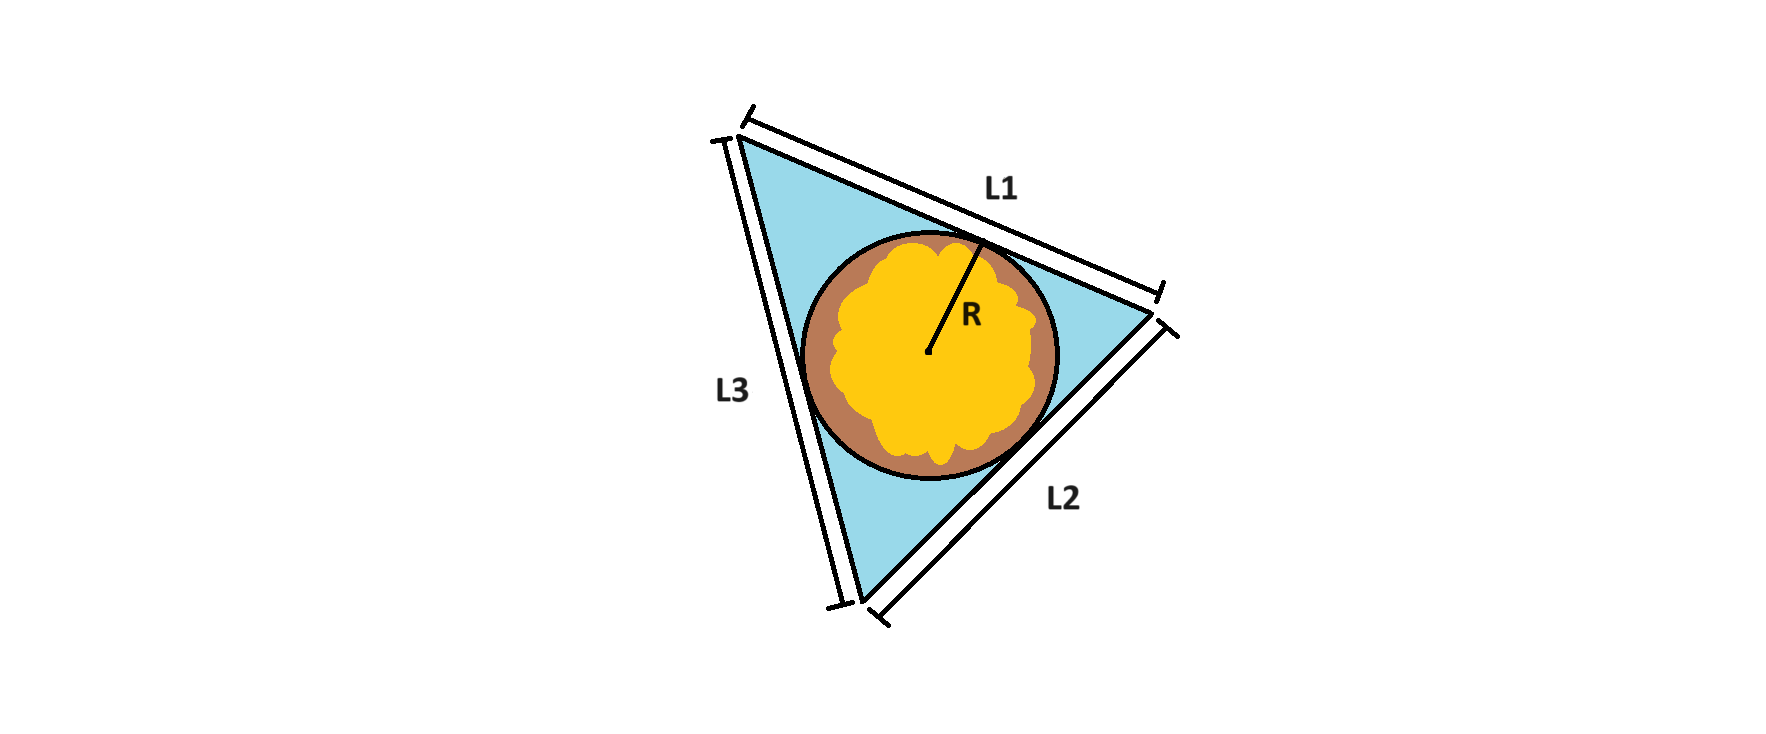
\includegraphics[scale=0.5]{vasilhaerrada.png}
\end{figure}

\subsection*{Entrada}
 
A primeira linha da entrada contém o número $N$ ($1\leq N\leq 1000$) de vasilhas.
 
As próximas $N$ linhas conterá os valores de $L1, L2, L3$ ($1\leq L1, L2, L3 \leq 500$) em cm representando as medidas realizadas por Nathan em cada recipiente. Considere que Nathan não erre as medidas e que a precisão pode alcançar duas casas decimais.
 
\subsection*{Saída}
A saída deverá conter $N$ números, sendo um valor por linha, que serão os raios R máximos, com duas casas decimais, que a panqueca pode ter em cada vasilha apresentado por Nathan.

%----- Exemplo 1 -----%
%\newpage
\begin{table}[!h]
\centering
\begin{tabular}{|l|l|}
\hline
\begin{minipage}[t]{3in}
\textbf{Exemplo de entrada}
\begin{verbatim}
6
3 4 5
12 12 12
10 12 10
2.08 1.82 1.30
33.07 96.2 103.86
131.27 316.33 216.7
\end{verbatim}
\vspace{1mm}
\end{minipage}
&
\begin{minipage}[t]{3in}
\textbf{Exemplo de saída}
\begin{verbatim}
1.00
3.46
3.00
0.45
13.61
33.24
\end{verbatim}
\vspace{1mm}
\end{minipage} \\
\hline
\end{tabular}
\end{table}
